\documentclass{utmreport}
\newcommand{\ReportTitle}{DES Key Permutation and Subkey Initialization}
\newcommand{\ReportSubtitle}{\ReportCourse: Task 2.1, student number 12}
% Load after defining ReportTitle; optional per-report settings follow below.
% Shared identity and course details for all laboratory reports.
\student{Gafenco Victor}{FAF-241}
\supervisor{asist. univ. Zaica Maia}{}
\newcommand{\ReportCourse}{Cryptography}
\cityyear{Chișinău}{2026}
\institution{Technical University of Moldova}
\faculty{Faculty of Computers, Informatics, and Microelectronics}
\department{Department of Software Engineering}
\studyprogramme{Software Engineering Study Programme}
\newcommand{\repositoryurl}{https://github.com/yoda-dinmd/crypt-labs}

\providecommand{\ReportNumber}{\expandafter\ReportNumberFromJob\jobname\relax}
\def\ReportNumberFromJob#1#2#3#4\relax{#4}
\providecommand{\ReportSubtitle}{}
\selectlanguage{english}
\ifPDFTeX\else\setmonofont{Liberation Mono}\fi
\utmlogo{../latex/assets/UTM_Logo_English.jpeg}
\documenttype{Laboratory report no. \ReportNumber}
\reporttitle{\ReportTitle}
\reportsubtitle{\ReportSubtitle}
\hypersetup{
  pdftitle={\ReportTitle},
  pdfauthor={\UTMStudentName},
  pdfsubject={\ReportCourse{} laboratory report no. \ReportNumber}
}

% Shared wording for references to the supplied Cryptography handouts.
% Arguments: laboratory number, topic, optional descriptive text (including punctuation).
\newcommand{\ReportHandoutReference}[3]{%
  \textit{Laboratory Work No. #1. #2}. Supplied course handout#3}

\lstset{language=Java}
\begin{document}
\makeutmreporttitlepage
\tableofcontents
\clearpage
\begin{utmabstract}[Abstract]
This laboratory examines the key initialization stage of the Data Encryption Standard (DES) block cipher and implements Task 2.1 in Java. For student number $n=12$, the task index is $12\bmod11=1$, which requires deriving the 56-bit permuted key $K^+$ from an 8-symbol key. Each printable American Standard Code for Information Interchange (ASCII) character is encoded as an 8-bit binary byte to form the 64-bit key $K$. Permuted Choice 1 (PC-1) then discards the eight byte-parity bits at positions $8,16,24,32,40,48,56$ and $64$, and rearranges the remaining 56 bits into the two 28-bit registers $C_0$ and $D_0$ that compose $K^+$. The console application supports both manual entry and random key generation, prints all tables used and every intermediate bit selection, and is verified by automated JUnit tests.
\utmkeywords{Data Encryption Standard, block cipher, key schedule, Permuted Choice 1, ASCII encoding, Java}
\end{utmabstract}

\utmintroduction
The objective of this laboratory work is to study the structure of the Data Encryption Standard (DES) symmetric block cipher and implement Task 2.1 for student order number $n=12$ ($n\bmod11=12\bmod11=1$). Task 2.1 requires determining the 56-bit permuted key $K^+$ from an 8-symbol DES key.

The application allows the user either to enter an 8-symbol ASCII key manually or to generate one randomly, validates the input, and displays on the screen all tables used together with every intermediate step of the transformation \cite{repo}.

\chapter{Short theory}
The Data Encryption Standard (DES) is a symmetric-key Feistel block cipher that encrypts 64-bit plaintext blocks under the control of a 64-bit key block, of which 56 bits participate directly in the cryptographic transformations.

\section{Structure of the DES algorithm}
Encryption of a 64-bit plaintext block $M$ proceeds through three main stages:
\begin{itemize}
\item an Initial Permutation (IP) rearranges the 64 bits of $M$ and splits the result into a 32-bit left half $L_0$ and a 32-bit right half $R_0$;
\item sixteen identical Feistel rounds ($i=1,\ldots,16$) update the halves according to:
\begin{equation}
L_i = R_{i-1},\qquad R_i = L_{i-1}\oplus f(R_{i-1}, K_i),
\end{equation}
where $\oplus$ denotes bitwise exclusive OR (XOR) and $K_i$ is the 48-bit round subkey;
\item after round 16, the swapped 64-bit pre-output $R_{16}L_{16}$ is passed through the final permutation $\text{IP}^{-1}$ to produce the 64-bit ciphertext block $C$;
\end{itemize}

Inside each round $i$, the Feistel function $f(R_{i-1},K_i)$ expands the 32-bit half $R_{i-1}$ to 48 bits via the expansion table $E$, computes $E(R_{i-1})\oplus K_i = B_1B_2B_3B_4B_5B_6B_7B_8$ as eight 6-bit blocks, compresses each 6-bit block $B_j$ to 4 bits through substitution box $S_j$ (using the outer two bits for the row index $0\ldots3$ and the inner four bits for the column index $0\ldots15$), and permutes the concatenated 32-bit output $S_1(B_1)\cdots S_8(B_8)$ through the straight permutation table $P$. Decryption uses the identical circuit with the round subkeys applied in reverse order ($K_{16}$ down to $K_1$).

\section{Key encoding and Permuted Choice 1 (PC-1)}
The DES key schedule derives the sixteen 48-bit round keys $K_1,\ldots,K_{16}$ from an initial 8-symbol key $K=s_1s_2s_3s_4s_5s_6s_7s_8$. Each symbol $s_j$ ($j=1,\ldots,8$) is converted via its ASCII code into an 8-bit binary byte, ordered from most significant bit (MSB) to least significant bit (LSB). Concatenating the eight bytes yields the 64-bit key block:
\begin{equation}
K = k_1k_2k_3\ldots k_{64},
\end{equation}
where byte $j$ occupies bit positions $8(j-1)+1$ through $8j$. The eighth bit of every byte ($k_8,k_{16},k_{24},k_{32},k_{40},k_{48},k_{56},k_{64}$) serves as a parity position and is ignored by the key schedule.

The first step of the key schedule applies Permuted Choice 1 (PC-1), given in Table~\ref{tab:pc1}, to select and reorder the 56 non-parity bits of $K$:
\begin{equation}
K^+ = k_{\text{PC-1}(1)}\,k_{\text{PC-1}(2)}\,\ldots\,k_{\text{PC-1}(56)} = C_0 D_0.
\end{equation}
\begin{table}[!htbp]
\caption{Permuted Choice 1 (PC-1) bit selection table}
\label{tab:pc1}\centering
\begin{tabular}{crrrrrrr}\hline
Half & \multicolumn{7}{c}{Source bit positions in the 64-bit key $K$}\\\hline
$C_0$ (bits 1--7)   & 57 & 49 & 41 & 33 & 25 & 17 &  9\\
$C_0$ (bits 8--14)  &  1 & 58 & 50 & 42 & 34 & 26 & 18\\
$C_0$ (bits 15--21) & 10 &  2 & 59 & 51 & 43 & 35 & 27\\
$C_0$ (bits 22--28) & 19 & 11 &  3 & 60 & 52 & 44 & 36\\\hline
$D_0$ (bits 29--35) & 63 & 55 & 47 & 39 & 31 & 23 & 15\\
$D_0$ (bits 36--42) &  7 & 62 & 54 & 46 & 38 & 30 & 22\\
$D_0$ (bits 43--49) & 14 &  6 & 61 & 53 & 45 & 37 & 29\\
$D_0$ (bits 50--56) & 21 & 13 &  5 & 28 & 20 & 12 &  4\\\hline
\end{tabular}
\end{table}

The first four rows of Table~\ref{tab:pc1} form the 28-bit left register $C_0$ by reading bit columns 1, 2 and 3 of the eight key bytes from byte 8 up to byte 1, followed by column 4 of bytes 8 through 5. The last four rows form the 28-bit right register $D_0$ by reading columns 7, 6 and 5 from byte 8 up to byte 1, followed by column 4 of bytes 4 through 1. In subsequent stages of the DES key schedule, $C_{i-1}$ and $D_{i-1}$ undergo circular left shifts of one bit (in rounds $1,2,9,16$) or two bits (in all other rounds), and Permuted Choice 2 (PC-2) selects 48 bits from $C_iD_i$ to form each round key $K_i$.

\chapter{Implementation}
The Java implementation is organized in the \texttt{md.utm.cryptography.lab4} package and separates the cryptographic key transformation from the interactive console interface \cite{repo}.

\section{ASCII encoding and key validation}
\texttt{DesKeyPermutation} validates 8-symbol keys, supports random generation over printable alphanumeric ASCII characters, and converts each symbol into an 8-bit binary string. Validation inspects every Unicode code point to reject control characters and non-ASCII symbols outside the printable range \texttt{U+0020}--\texttt{U+007E}, and verifies that the key length is exactly 8 characters:
\begin{lstlisting}
public static String toBinaryKey(String key) {
    String validated = validateKey(key);
    StringBuilder bits = new StringBuilder(64);
    for (int i = 0; i < validated.length(); i++) {
        bits.append(toEightBitBinary(validated.charAt(i)));
    }
    return bits.toString();
}
\end{lstlisting}
Each character code is formatted with \texttt{Integer.toBinaryString} and left-padded with zeros to 8 bits, preserving the bit numbering from $k_1$ (MSB of byte 1) to $k_{64}$ (LSB of byte 8).

\section{PC-1 permutation and intermediate trace}
The constant array \texttt{PC1} stores the 56 one-based bit positions from Table~\ref{tab:pc1}. The method \texttt{applyPc1} verifies that the input string contains 64 binary digits and maps each one-based position \texttt{PC1[j]} to zero-based string index \texttt{PC1[j] - 1}:
\begin{lstlisting}
public static String applyPc1(String binaryKey) {
    if (binaryKey == null || binaryKey.length() != 64
            || !binaryKey.chars().allMatch(ch -> ch == '0' || ch == '1')) {
        throw new IllegalArgumentException(
                "Binary key K must contain exactly 64 bits ('0' or '1').");
    }
    StringBuilder permuted = new StringBuilder(PC1.length);
    for (int position : PC1) {
        permuted.append(binaryKey.charAt(position - 1));
    }
    return permuted.toString();
}
\end{lstlisting}
The methods \texttt{c0()} and \texttt{d0()} return the 28-bit halves \texttt{kPlus.substring(0, 28)} and \texttt{kPlus.substring(28, 56)}. The method \texttt{formatTrace()} builds the complete console report: the byte-by-byte ASCII and binary breakdown table (highlighting the 7 data bits and the 8th parity bit of each byte), the 64-bit key $K$ in hexadecimal and 8-bit blocks, the 8-row PC-1 table paired with every intermediate bit lookup $k_{\text{PC-1}(j)}$, and the resulting registers $C_0$, $D_0$ and $K^+$.

\section{Console interface and build integration}
\texttt{Main} provides an interactive loop with three options: manual 8-symbol key entry (\texttt{1}), random 8-symbol key generation (\texttt{2}), and exit (\texttt{0}). Random keys are generated with \texttt{SecureRandom} during interactive use, while an optional \texttt{-Dlab4.seed} system property enables deterministic regeneration of console transcripts. Invalid menu selections or malformed keys display an explanation and retry the current prompt without terminating the session. The \texttt{lab4} Maven module compiles under the root aggregator and packages an executable JAR with \texttt{md.utm.cryptography.lab4.Main} as its entry point.

\chapter{Results and verification}
The implementation is verified through a step-by-step worked example, captured console sessions for manual, random and invalid inputs, and automated unit tests.

\section{Worked example for an 8-symbol key}
For the 8-symbol ASCII key \texttt{CRYPTO26}, Table~\ref{tab:ascii} gives the byte-level encoding into the 64-bit key $K$.
\begin{table}[!htbp]
\caption{ASCII and binary representation of the 8-symbol key \texttt{CRYPTO26}}
\label{tab:ascii}\centering
\begin{tabular}{ccrcccr}\hline
Byte & Symbol & ASCII (dec / hex) & Bit range & 8-bit binary & Data bits (1--7) & Parity bit\\\hline
1 & \texttt{C} & 67 / \texttt{0x43} & 1--8   & \texttt{01000011} & \texttt{0100001} & $k_{8}=1$\\
2 & \texttt{R} & 82 / \texttt{0x52} & 9--16  & \texttt{01010010} & \texttt{0101001} & $k_{16}=0$\\
3 & \texttt{Y} & 89 / \texttt{0x59} & 17--24 & \texttt{01011001} & \texttt{0101100} & $k_{24}=1$\\
4 & \texttt{P} & 80 / \texttt{0x50} & 25--32 & \texttt{01010000} & \texttt{0101000} & $k_{32}=0$\\
5 & \texttt{T} & 84 / \texttt{0x54} & 33--40 & \texttt{01010100} & \texttt{0101010} & $k_{40}=0$\\
6 & \texttt{O} & 79 / \texttt{0x4F} & 41--48 & \texttt{01001111} & \texttt{0100111} & $k_{48}=1$\\
7 & \texttt{2} & 50 / \texttt{0x32} & 49--56 & \texttt{00110010} & \texttt{0011001} & $k_{56}=0$\\
8 & \texttt{6} & 54 / \texttt{0x36} & 57--64 & \texttt{00110110} & \texttt{0011011} & $k_{64}=0$\\\hline
\end{tabular}
\end{table}

Because every standard 7-bit ASCII code lies below 128, the most significant bit of each byte ($k_1,k_9,k_{17},k_{25},k_{33},k_{41},k_{49},k_{57}$) equals \texttt{0}. Applying Table~\ref{tab:pc1} extracts those eight bits first into $C_0$, yielding:
\begin{align}
C_0 &= \texttt{0000000 0001111 1111000 0001101},\\
D_0 &= \texttt{1110001 1101100 0000100 1001110},\\
K^+ &= \texttt{0000000 0001111 1111000 0001101 1110001 1101100 0000100 1001110}.
\end{align}

\section{Console evidence}
Figures~\ref{fig:manual}, \ref{fig:random} and \ref{fig:invalid} show executable-JAR console sessions captured through a pseudo-terminal. They can be regenerated after building with:
\begin{lstlisting}[language={}]
python3 scripts/capture-results.py --lab lab4
\end{lstlisting}
Figure~\ref{fig:manual} demonstrates manual input of the 8-symbol key \texttt{CRYPTO26}, displaying the ASCII encoding table, the PC-1 table, the intermediate bit selections, and the resulting 56-bit key $K^+$.
\begin{figure}[!htbp]
\centering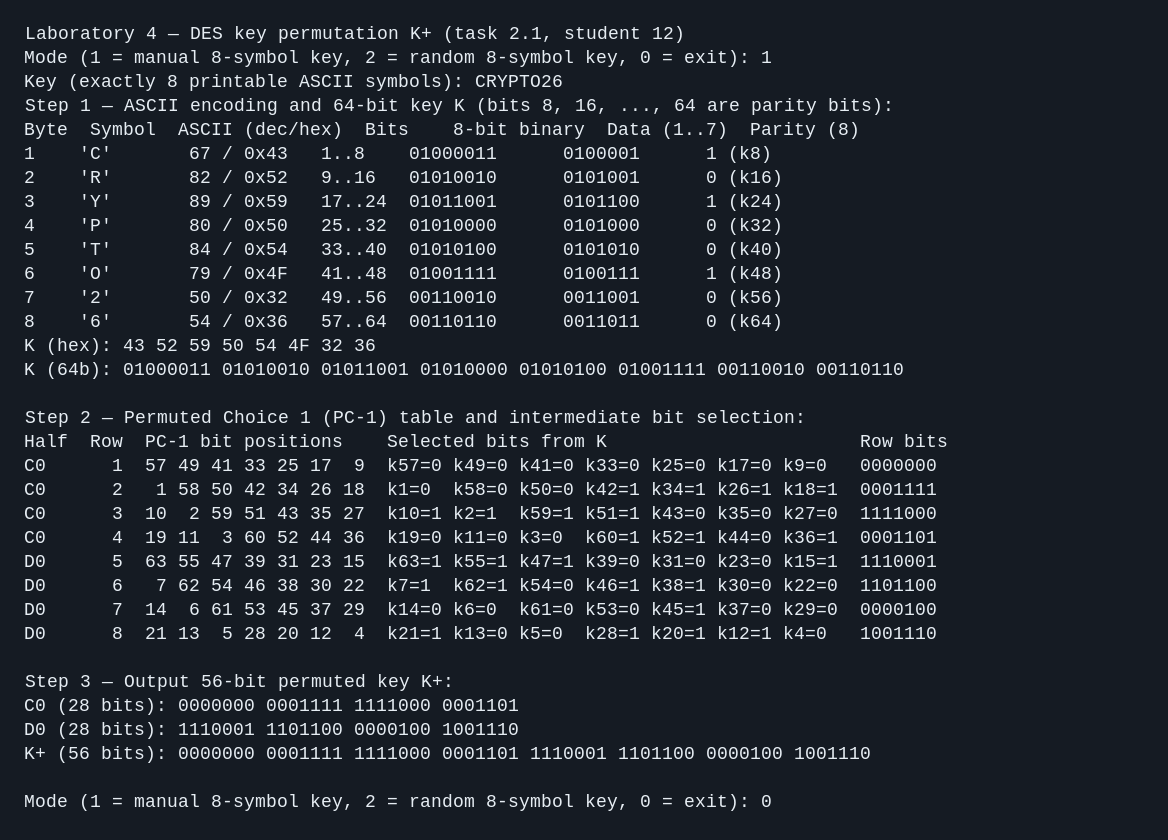
\includegraphics[width=\textwidth]{screenshots/manual.png}
\caption{Manual 8-symbol key entry and intermediate PC-1 trace}\label{fig:manual}
\end{figure}
\clearpage
Figure~\ref{fig:random} shows mode \texttt{2}, where the program generates the random 8-symbol key \texttt{Q4G5wDqb} and computes $K^+=\texttt{0000000 0111101 0111011 0100101 1001010 0001111 1000000 0001011}$.
\begin{figure}[!htbp]
\centering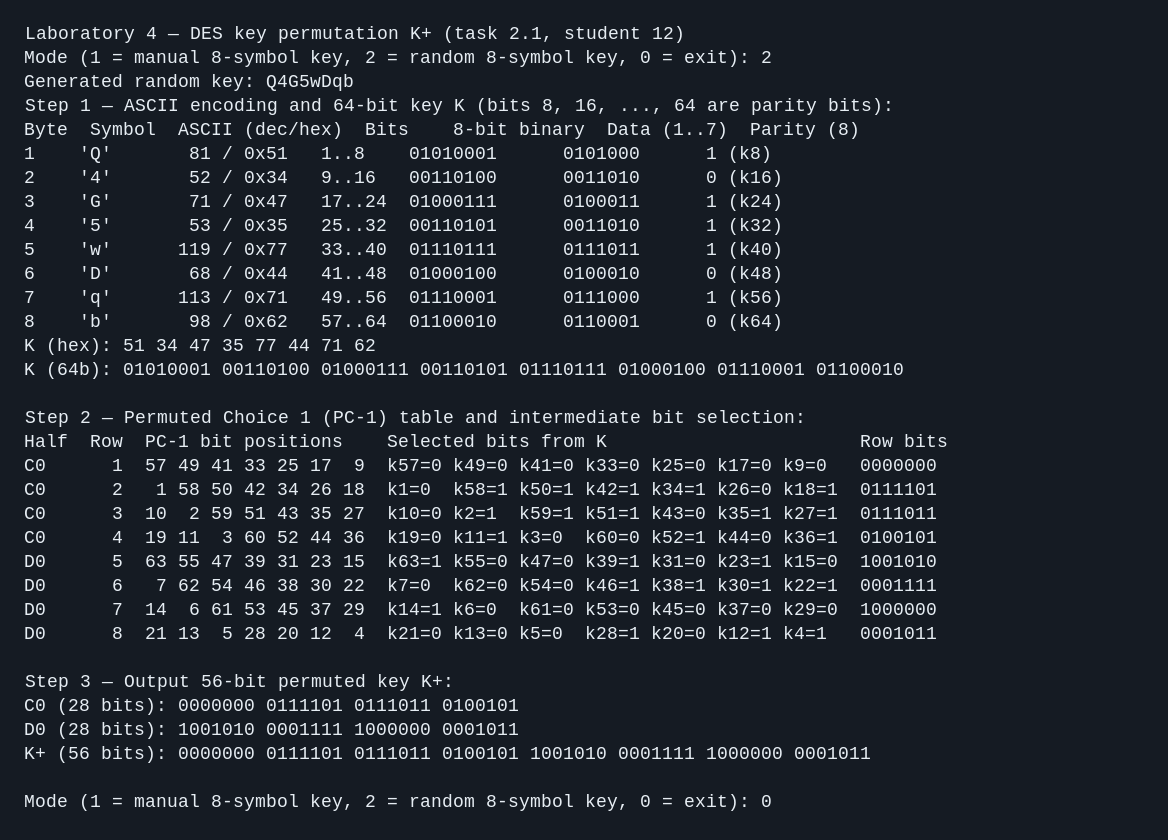
\includegraphics[width=\textwidth]{screenshots/random.png}
\caption{Random 8-symbol key generation and derivation of $K^+$}\label{fig:random}
\end{figure}

Figure~\ref{fig:invalid} demonstrates input validation: the program rejects menu option \texttt{3}, a 5-character key (\texttt{SHORT}), a 10-character key (\texttt{TOOLONGKEY}), and a key containing a non-ASCII character (\texttt{Română12}), before accepting \texttt{DESKEY01}.
\begin{figure}[!htbp]
\centering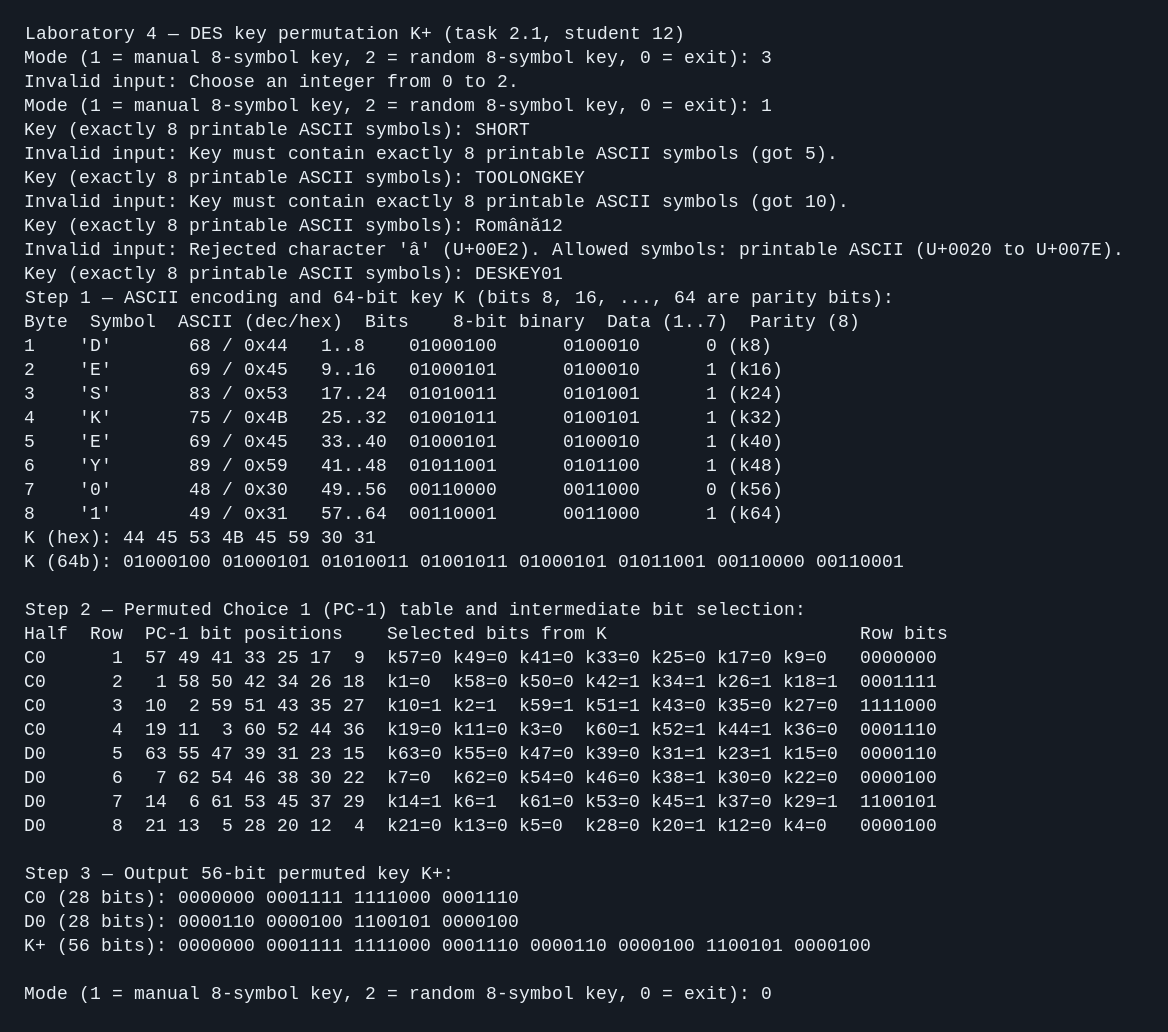
\includegraphics[width=\textwidth]{screenshots/invalid.png}
\caption{Validation of menu choices, key length and non-ASCII characters}\label{fig:invalid}
\end{figure}

\section{Automated verification}
Five JUnit tests in \texttt{DesKeyPermutationTest} verify the implementation:
\begin{itemize}
\item comparison against the standard 64-bit hexadecimal test vector \texttt{133457799BBCDFF1}, confirming that \texttt{applyPc1} produces $C_0=\texttt{1111000 0110011 0010101 0101111}$ and $D_0=\texttt{0101010 1011001 1001111 0001111}$;
\item verification of the complete ASCII-to-$K^+$ pipeline and formatted trace for \texttt{CRYPTO26};
\item exhaustive structural testing across all 56 unit-bit vectors, proving that PC-1 is a bijection from $\{1,\ldots,64\}\setminus\{8,16,24,32,40,48,56,64\}$ onto $\{1,\ldots,56\}$ and that setting all eight parity bits to \texttt{1} yields an all-zero $K^+$;
\item verification of 25 randomly generated 8-symbol keys;
\item rejection of \texttt{null}, wrong-length keys, non-ASCII characters, control characters, and malformed 64-bit binary strings;
\end{itemize}

\utmconclusions
Task 2.1 of Laboratory Work No.~4 is implemented in Java, converting any 8-symbol printable ASCII key into its 64-bit binary representation $K$ and applying Permuted Choice 1 (PC-1) to obtain the 56-bit permuted key $K^+=C_0D_0$. Displaying the byte-level ASCII table alongside the row-by-row PC-1 bit selections makes both parity-bit removal and cross-byte bit transposition explicit.

The experiment also highlights an important practical property of ASCII-entered DES keys: because standard 7-bit ASCII characters always have a zero most significant bit in every byte ($k_1,k_9,\ldots,k_{57}=0$) while the eighth bit ($k_8,k_{16},\ldots,k_{64}$) is discarded by PC-1, an 8-character printable ASCII key supplies at most $8\times6=48$ variable bits out of the 56 bits in $K^+$, with the first eight bits of $C_0$ fixed to zero.

\begin{thebibliography}{9}
\bibitem{repo} Gafenco Victor. \textit{Cryptography Laboratory Repository} [online]. GitHub, 2026 [accessed 09.11.2026]. Available: \url{\repositoryurl}
\end{thebibliography}
\end{document}
